\documentclass[../../Main/Main.tex]{subfiles}

\begin{document}

\chapter{Role of the models in statistical mechanics}
\section{Role of the models}
Which is the role of models in statistical mechanics? There are two possible approaches:
\begin{enumerate}
  \item The model must describe the real system in a very detailed way. The maximum number of details and parameters to be tuned are included. The \emph{pro} is the closer to the real specific system (faithfull description). The \emph{drawback} is that the model is so complicated that no analytical solution is possible. Moreover, even numerically, these models can be studied for very short times and small sizes.
  An example is the simulation of the folding dynamics that can be performed for few nanoseconds. On the other hand, the introduction of many details are often not crucial if one is interested in large scale properties.
  \item Try to introduce (coarse-graining approach) the most simple model that satisfies few essential properties of the real system such as its symmetries, dimensionality, range of interactions etc.
  Since most of the microscopic details are integrated, these models cannot describe the full physics of a specific system but they can reproduce its main features. Moreover, these models can be studied numerically and, to some extent, also analytically (exact solution).
\end{enumerate}

It is the latter approach that we shall take here.
  Let us start by introducing what is, perhaps, the most paradigmatic model in the statistical mechanics of phase transition, the \emph{Ising model}.

  \section{The Ising model}
  Suggested by Lenz to Ising for his PHD thesis (1925), it is supposed to describe a magnetic system that undergoes a transition between a paramagnetic and a ferromagnetic phase.
  In \( d=1 \) the model was solved exactly by Ising. Unfortunately, he found that for \( T>0 \) the model does not display a phase transition.

  The wrong conclusion was that this model was not able to describe a phase transition. In fact, it turns out that, for \( d>1 \), the model does display a paramagnetic-ferromagnetic phase transition.

   Let us first discuss some general feature of the model for any dimension \( d \).

\subsection{\emph{d}-dimensional Ising model}
For hypercubic lattice with  given \( N(\Omega ) \) sites \( \{ i \}_{i=1,\dots,N(\Omega )}   \) and linear size \( L(\Omega ) \), we have
\begin{equation*}
   N (\Omega ) = L^d
\end{equation*}
 The microscopic degrees of freedom are the spins \( S_i \), defined at each \emph{i}-esim lattice site. Each spin can assume the values  \( S_i = \pm 1 \), that means that at each site the possible values are the spin up or down.
 For a lattice with \( N(\Omega ) \) spins, there are \( 2^{N(\Omega )} \)  possible configurations.
 \begin{remark}
 Since we do not consider the spin as a vector, this is a model for a strongly anysotropic ferromagnet (along a given direction).
 \end{remark}
 The minimal model that can try to capture the interaction between the spin is the following.
Suppose to have also an external magnetic field \( H_i \) (it values depends on the site \emph{i}). One can consider interactions between spins whose strength are described by functions \( J_{ij},k_{ijk}, \dots \). For instance, there is a coupling that derives from electrons coupling
\begin{equation*}
  J_{ij} = f ( \abs{\va{r_i}- \va{r_j}  } )
\end{equation*}
The physical origin is the overlap between the electronic orbitals of the neighbouring atoms forming the Bravais lattice.
Remember that a term as \( \sum_{i}^{} S_i  \) is not correlated, while we need an interaction for describing the model.

A general Hamiltonian of the model can be written as:
\begin{equation*}
  \mathcal{H}_ \Omega ( \{ S_i \}  ) = \sum_{ij}^{} J_{ij} S_i S_j - \sum_{i}^{} H_i S_i - \sum_{ijk}^{} S_i S_j S_k + \dots
\end{equation*}
Standard Ising model one keeps only the two-body interactions:
\begin{empheq}[box=\myyellowbox]{equation}
  \mathcal{H}_ \Omega ( \{ S_i \}  ) = -\frac{1}{2}\sum_{i,j}^{N} J_{ij} S_i S_j - \sum_{i=1}^{N} H_i S_i
\end{empheq}
where the first term represents a two body interaction that is a quadratic term, while the second term is a one body interaction.  We have put the minus because we want to minimize the energy, but it depends on the sign of  \emph{J}.

For this model, the sum over all configurations on trace is given by
\begin{equation*}
  \Tr \equiv \sum_{S_1 = \pm 1}^{}  \sum_{S_2 = \pm 1}^{}  \dots \sum_{S_N = \pm 1}^{} \equiv \sum_{\{ S \}  }^{}
\end{equation*}
 Our problem is to find the partition function with \emph{N} sites, which depends on \emph{T} and in principle depends on the configuration given (it is fixed both for \emph{H} and \emph{J}!).
Hence, the \emph{canonical partition function} is given by
\begin{equation}
  Z_{\Omega } (T, \{ H_i \}, \{ J_{ij} \}    ) = \Tr e^{-\beta \mathcal{H}_ \Omega ( \{ S \}  )}
\end{equation}
and the corresponding \emph{free-energy},
\begin{equation}
  F_ \Omega  (T, \{ H_i \}, \{ J_{ij} \} ) = - k_B T \ln{Z_ \Omega }
\end{equation}
The \emph{bulk limiting free energy} is:
\begin{equation}
  f_b (T, \{ H_i \}, \{ J_{ij} \} ) = \lim_{N \rightarrow \infty }\frac{1}{N}  F_ \Omega  
\end{equation}
How do we know that the above limit does exist? It must be proven. The surface is not important in the bulk limit.
 Note that we are assuming that the \emph{interaction between the spin is a short range force}, it is not as the size of the system.

For this model it is possible to show that the limit exists if
\begin{equation}
  \sum_{j \neq i}^{} \abs{J_{ij}} < \infty
\end{equation}
\begin{remark}
In general what determines the existence of the limit of these spin models are the \emph{dimension} \emph{d} and the \emph{range} of the spins \emph{interactions}.
\end{remark}
For example it is possible to show that, if
\begin{equation}
  J_{ij} = A \abs{\va{r_i}-\va{r_j}  }^{-\sigma}
\end{equation}
so it is a long range interaction, the limit exists when
\begin{equation*}
  \sigma > d
\end{equation*}
\begin{remark}
If the interaction is \emph{dipolar}, since it decades as \( 1/r^3 \), for the case \( d=3 \) the limit does not exists. However, it is still possible to prove the existence of the limit for this case if one assumes that not all dipoles are fully aligned.
\end{remark}
Assuming that the thermodynamic limit exists, we now look at some additional rigorous results on the limiting free energy and its derivatives.

%%%%%%%%%%%%%% ADDED IN 2023 %%%%%%%%%%%%%%%%

\subsection{Thermodynamic Limit}

For simplicity, let us consider the case in which the external magnetic field is homogeneous, i.e. \( H_i \equiv H \), and the spin-spin interaction is only between spins that are nearest-neighbours (n.n.) on the lattice:
\begin{equation}
J_{ij} =
  \begin{cases}
  J & \text{if } i \text{ and } j \text{ are n.n.} \\
  0 & \text{otherwise}
  \end{cases}
\end{equation}
Now, the model is very simple:
\begin{equation}
  - \mathcal{H}_ \Omega ( \{ S \}  ) = J \sum_{\expval{ij} }^{N (\Omega )} S_i S_j + H \sum_{i}^{N(\Omega )} S_i
  \label{eq:6_0}
\end{equation}
where the notation \( \expval{ij}  \) means a double sum over \emph{i} and \emph{j}, with the constraint that \emph{i} and \emph{j} are nearest-neighbours.

To prove the existence of the thermodynamic limit of the Ising Model let us consider the case in which $H_{i} = H = 0$ for all nodes.
So our Hamiltonian becomes:
$$\mathcal{H}_{N}(\{ s \}) = -J \sum_{\avg{{ij}}} s_{i}s_{j}$$
To simplify the drawing let us prove it for $d=2$.

\begin{proof}
Given a square lattice with $N= 4n^{2}$ spins let us partition it into $4$ identical subsystems each with $n^{2}$ spins:

\begin{figure}[h!]
\centering
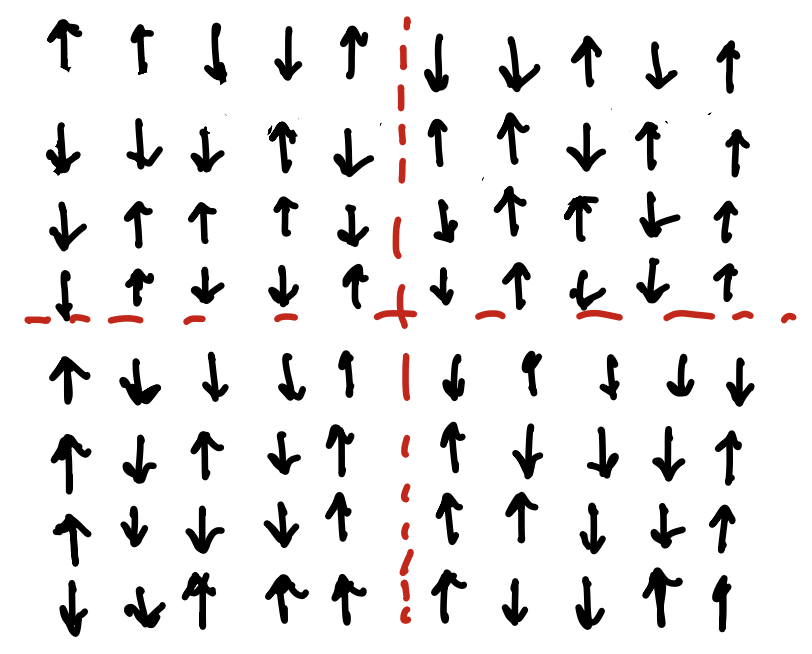
\includegraphics[width=0.6\textwidth]{./img/IMAGE1.png}
\end{figure}


If we neglect the surface interaction between the 4 subsystems we make an error in the estimate of the total energy ranging between $-4Jn$ (boundary spins are all parallel) and $4Jn$ (boundary spins are all anti-parallel).
Since the number of configurations is not modified by this partition if we assume that the subsystems are independent:
$$
(Z_{n^{2}})^{4} e^{-4\beta J{n}} \leq Z_{(2n)^{2}} \leq (Z_{n^{2}})^{4}e^{4\beta J{n}}
$$

With a free-energy density of a single subsystem:
$$f_{n^{2}} = -k_{B}T\ln\left( \frac{Z_{n^{2}}}{n^{2}} \right)$$
And for all the system:
$$f_{(2n)^{2}} = -k_{B}T\ln\left( \frac{Z_{(2n)^{2}}}{4n^{2}} \right)$$

By taking $k_{B}T\ln$ of the inequality above and dividing by the total "volume" $N = 4n^{2}$ we have
$$\frac{4}{\beta} \ln\left( \frac{Z_{n^{2}}}{4n^{2}} \right) - \frac{4\beta J_{n}}{\beta 4n^{2}} \leq f_{(2n)^{2}} \leq \frac{4\ln(Z_{n^{2}})}{\beta 4 n^{2}} + \frac{4\beta J_{n}}{\beta 4n^{2}}$$
Hence 
$$f_{n^{2}} - \frac{J}{n} \leq f_{(2n)^{2}} \leq f_{n^{2}} + \frac{J}{n}$$
That can be written has:
$$\mid f_{(2n)^{2}} - f_{n^{2}}\mid \leq \frac{\const}{n} =\const \cdot \frac{n}{n^{2}} \sim \frac{L}{S}$$

With $L =n$ as the "perimeter" and $S = n^{2}$ as the area. The difference is due to boundary effects.
If $f_{n^{2}}$ satisfies the last inequality it is a Cauchy Sequence so it converges to a finite limit.

The argument is easy to generalise to any dimensions: if $d=3$ consider a cube of $8N^{3}$ spins and partition it into $8$ sub-cubes, each of volume $N^{3}$ so $\frac{L}{S}$ becomes $\frac{S}{V}$.
\end{proof}
\begin{remark}
If $\mathcal{H}(\{ s \}) = -\frac{J}{2} \sum_{{i,j}} s_{i}s_{j}$ where the sum is over all pairs independently of their distance at $T = 0$ all the spins are aligned and $E \sim n^{4}$ so our limit becomes $\lim_{ n \to \infty } \frac{E}{n^{2}} \sim n^{2} \to \infty$
\end{remark}




%%%%%%%%%%%%%%%%%%%%%%%%%%%%%%%%%%%%%%%%%%%













\subsection{Order Parameter of the Ising Model}
%%%%%%%%%%%%%%% ADDED IN 2023 %%%%%%%%%%%%%%
Let us start again from the Hamiltonian: 
$$  - \mathcal{H} ( \{ S \}  ) = J \sum_{\expval{ij} }^{N} S_i S_j + H \sum_{i}^{N} S_i $$
One can formally express the Average Total Magnetization as
$$M = \avg{\sum_{i=1}^N S_i}$$
In the case in which $H$ is uniform we have
$$M(\beta) = \avg{\sum_{i=1}^{N}s_{i}} =   \frac{1}{Z_{N}}\Tr_{\{ s \}}\left( \sum_{i}s_{i} \right)e^{-\beta \mathcal{H}_{N}} = \frac{1}{\beta} \frac{ \partial \ln(Z_{N}) }{ \partial H  }\bigg\rvert_{\beta} $$

With $Z_{N}$ the generating function.
In general one is interested in the magnetisation density or per spins, so
$$m(\beta,H) = \frac{M(\beta,H)}{N} = \frac{1}{N\beta} \frac{ \partial \ln(Z_{N}) }{ \partial H  }\bigg\rvert_{\beta} = -\frac{1}{N} \frac{ \partial F_{N} }{ \partial H  }\bigg\rvert_{\beta} = -\frac{ \partial f_{N} }{ \partial H  }\bigg\rvert_{\beta} $$
With $m(\beta,H)$ being the \textbf{Order Parameter} of the Ising Model.

Note that for $H_{i} = H$, $m$ does not depend on $i$ (it's homogeneous) and, since $M = \sum_{i}s_{i}$ the partition function $$Z_{N}(\beta,J,H) = \Tr_{\{ s \}} \exp\left( \beta J \sum_{\avg{ {ij}}}s_{i}s_{j} + \beta HM \right)$$
coincides with the Gibbs partition function (and $f_{n}$ with the finite size Gibbs free-energy density $g_N$).

%%%%%%%%%%%%%%%%%%%%%%%%%%%

\subsection{Ising model and \( \mathbb{Z}^2 \) symmetry. }
The symmetry of the system in sense of the Hamiltonian is: we can invert the value of the \emph{S} and the Hamiltonian does not change. It is valid when \( H=0 \), otherwise it is not true. Let us see the \( \mathbb{Z}^2 \) symmetry and the following interesting relation:

  \begin{lemma}{}{}
  \( \forall  \) function \( \Phi  \) of the configuration \( \{ S_i \}   \), the following relation holds:
  \begin{equation}
    \sum_{ \{S_i = \pm 1\}}^{}  \Phi  (\{S_i\} ) =   \sum_{ \{S_i = \pm 1\}}^{}  \Phi  (\{-S_i\} )
      \label{eq:6_1}
  \end{equation}
  this is true for all function of the spin.
  \end{lemma}

Now, we consider the Hamiltonian of the Ising model:
\begin{equation*}
  - \mathcal{H}_ \Omega  = J \sum_{\expval{ij} }^{N(\Omega )} S_i S_j + H \sum_{i}^{N(\Omega )} S_i
\end{equation*}
Clearly,
\begin{equation}
  \mathcal{H}(H,J, \{S_i\}) =   \mathcal{H}_ \Omega (-H,J, \{-S_i\})
  \label{eq:6_1_1}
\end{equation}
This is a spontaneous broken symmetry.

Hence,
\begin{equation}
  \begin{split}
Z_ \Omega  (-H,J,T) &= \sum_{ \{S_i = \pm 1 \}}^{} \exp [-\beta \mathcal{H}_ \Omega  (-H,J, \{S_i\})]  \underset{\eqref{eq:6_1}}{=}   \sum_{ \{S_i = \pm 1 \}}^{} \exp [-\beta \mathcal{H}_ \Omega  (-H,J,\{-S_i\})] \\
&\underset{\eqref{eq:6_1_1}}{=} \sum_{ \{S_i= \pm 1\}}^{} \exp [-\beta \mathcal{H}_ \Omega  (H,J, \{S_i\}) ] = Z_ \Omega (H,J,T)
\end{split}
\end{equation}
Taking \( -k_B T \ln  \), we got:
\begin{equation}
  F_ \Omega  (T,J,H) = F_ \Omega  (T,J,-H)
  \label{eq:6_2}
\end{equation}
If we take the thermodynamic limit \( \lim_{N \rightarrow \infty } \frac{1}{N} \), we have
\begin{equation}
\Rightarrow f_b (T,J,H) = f_b (T,J,-H)
\end{equation}
and it means that the \emph{free energy density is an even function of H}!
\begin{remark}
From the finite-size relation \eqref{eq:6_2}, one can show that a \emph{finite-size}  Ising model does not display a transition to a ferromagnetic phase (for all dimension \emph{d}). Indeed,
\begin{equation}
    N (\Omega ) M(H) = - \pdv{F (H)}{H} \underset{\eqref{eq:6_2}}{=}  - \pdv{F(-H)}{(H)} = \pdv{F(-H)}{(-H)}  = - N (\Omega ) M (-H)
\end{equation}
Therefore:
\begin{equation}
  M (H) = - M (-H), \quad \forall H
\end{equation}
If \( H=0 \), we have \( M (0) = -M (0) \), that is valid if and only if \( M(0)= 0 \)!

The magnetization of a finite system is, at \( H=0 \), always zero. This is simply consequence of the symmetry argument shown above. We have not a phase transition.

Hence, it is only in the thermodynamic limit, where the symmetry is spontaneously broken, that the model displays a transition.

For resuming, although the Hamiltonian is invariant with respect to the transformation \( H \rightarrow -H, \{ S_i \} \rightarrow \{-S_i\} \), the thermodynamic state is not. This situation is called \emph{spontaneous symmetry breaking}.
\end{remark}
\end{document}
